%%%%%%%%%%%%%%%%%%%%%%%%%%%%%%%%%%%%%%%%%
% Short Sectioned Assignment LaTeX Template Version 1.0 (5/5/12)
% This template has been downloaded from: http://www.LaTeXTemplates.com
% Original author:  Frits Wenneker (http://www.howtotex.com)
% License: CC BY-NC-SA 3.0 (http://creativecommons.org/licenses/by-nc-sa/3.0/)
%%%%%%%%%%%%%%%%%%%%%%%%%%%%%%%%%%%%%%%%%

%----------------------------------------------------------------------------------------
%	PACKAGES AND OTHER DOCUMENT CONFIGURATIONS
%----------------------------------------------------------------------------------------

\documentclass[paper=a4, fontsize=11pt]{scrartcl} % A4 paper and 11pt font size

% ---- Entrada y salida de texto -----

\usepackage[T1]{fontenc} % Use 8-bit encoding that has 256 glyphs
\usepackage[utf8]{inputenc}
%\usepackage{fourier} % Use the Adobe Utopia font for the document - comment this line to return to the LaTeX default

% ---- Idioma --------

\usepackage[spanish, es-tabla]{babel} % Selecciona el español para palabras introducidas automáticamente, p.ej. "septiembre" en la fecha y especifica que se use la palabra Tabla en vez de Cuadro

% ---- Otros paquetes ----

\usepackage{amsmath,amsfonts,amsthm} % Math packages
%\usepackage{graphics,graphicx, floatrow} %para incluir imágenes y notas en las imágenes
\usepackage{graphics,graphicx, float} %para incluir imágenes y colocarlas

% Para hacer tablas comlejas
%\usepackage{multirow}
%\usepackage{threeparttable}

%\usepackage{sectsty} % Allows customizing section commands
%\allsectionsfont{\centering \normalfont\scshape} % Make all sections centered, the default font and small caps

\usepackage{fancyhdr} % Custom headers and footers
\usepackage{url}
\usepackage[hidelinks]{hyperref}
\pagestyle{fancyplain} % Makes all pages in the document conform to the custom headers and footers
\fancyhead{} % No page header - if you want one, create it in the same way as the footers below
\fancyfoot[L]{} % Empty left footer
\fancyfoot[C]{} % Empty center footer
\fancyfoot[R]{\thepage} % Page numbering for right footer
\renewcommand{\headrulewidth}{0pt} % Remove header underlines
\renewcommand{\footrulewidth}{0pt} % Remove footer underlines
\setlength{\headheight}{13.6pt} % Customize the height of the header

\DeclareOldFontCommand{\rm}{\normalfont\rmfamily}{\mathrm}
\DeclareOldFontCommand{\sf}{\normalfont\sffamily}{\mathsf}
\DeclareOldFontCommand{\tt}{\normalfont\ttfamily}{\mathtt}
\DeclareOldFontCommand{\bf}{\normalfont\bfseries}{\mathbf}
\DeclareOldFontCommand{\it}{\normalfont\itshape}{\mathit}
\DeclareOldFontCommand{\sl}{\normalfont\slshape}{\@nomath\sl}
\DeclareOldFontCommand{\sc}{\normalfont\scshape}{\@nomath\sc}
\DeclareRobustCommand*\cal{\@fontswitch\relax\mathcal}
\DeclareRobustCommand*\mit{\@fontswitch\relax\mathnormal}

\numberwithin{equation}{section} % Number equations within sections (i.e. 1.1, 1.2, 2.1, 2.2 instead of 1, 2, 3, 4)
\numberwithin{figure}{section} % Number figures within sections (i.e. 1.1, 1.2, 2.1, 2.2 instead of 1, 2, 3, 4)
\numberwithin{table}{section} % Number tables within sections (i.e. 1.1, 1.2, 2.1, 2.2 instead of 1, 2, 3, 4)

\setlength\parindent{0pt} % Removes all indentation from paragraphs - comment this line for an assignment with lots of text

\newcommand{\horrule}[1]{\rule{\linewidth}{#1}} % Create horizontal rule command with 1 argument of height




%----------------------------------------------------------------------------------------
%	TÍTULO Y DATOS DEL ALUMNO
%----------------------------------------------------------------------------------------

\title{	
\normalfont \normalsize 
\textsc{{\bf Visión por computador (2016-2017)} \\ Grado en Ingeniería Informática \\ Universidad de Granada} \\ [25pt] % Your university, school and/or department name(s)
\horrule{0.5pt} \\[0.4cm] % Thin top horizontal rule
\huge Memoria Práctica 2 \\ % The assignment title
\horrule{2pt} \\[0.5cm] % Thick bottom horizontal rule
}

\author{Ignacio Martín Requena} % Nombre y apellidos

\date{\normalsize\today} % Incluye la fecha actual

%----------------------------------------------------------------------------------------
% DOCUMENTO
%----------------------------------------------------------------------------------------
\usepackage{graphicx}
\usepackage{listings}
\usepackage{color}
\definecolor{gray97}{gray}{.97}
\definecolor{gray75}{gray}{.75}
\definecolor{gray45}{gray}{.45}
 

\lstset{ frame=Ltb,
     framerule=0pt,
     aboveskip=0.5cm,
     framextopmargin=3pt,
     framexbottommargin=3pt,
     framexleftmargin=0.4cm,
     framesep=0pt,
     rulesep=.4pt,
     backgroundcolor=\color{gray97},
     rulesepcolor=\color{black},
     %
     stringstyle=\ttfamily,
     showstringspaces = false,
     basicstyle=\small\ttfamily,
     commentstyle=\color{gray45},
     keywordstyle=\bfseries,
     %
     numbers=left,
     numbersep=15pt,
     numberstyle=\tiny,
     numberfirstline = false,
     breaklines=true,
   }
 


\lstdefinestyle{consola}
   {basicstyle=\scriptsize\bf\ttfamily,
    backgroundcolor=\color{gray75},
   }
 
\lstdefinestyle{C}
   {language=C,
   }



\begin{document}

\maketitle % Muestra el Título

\newpage %inserta un salto de página

\tableofcontents % para generar el índice de contenidos

\listoffigures

\newpage



%----------------------------------------------------------------------------------------
%	Cuestion 1
%----------------------------------------------------------------------------------------

\section{Ejercicio 1}

\subsection{Enunciado}
 Escribir una función que extraiga la lista potencial de puntos Harris en una imagen a distintas escalas. Para ello construiremos una pirámide Gaussiana de la imagen con 4 escalas usando sigma=1. Sobre cada nivel de la pirámide usar la función OpenCV cornerHarris que devuelve el mapa de valores del criterio Harris en cada píxel. Seleccionar al menos los 1500 puntos de entre los de mayor valor distribuidos entre las distintas escalas (las escalas más bajas tendrán más puntos: 70-20-10). Mostrar el resultado identificando con un círculo o una cruz sobre la imagen original las coordenadas de los puntos seleccionados (ver circle()). (1.5 puntos)\\
 \\
 a. Calcular la orientación relevante de cada punto Harris, usando un alisamiento fuerte de las derivadas en x e y de las imágenes, en la escala correspondiente, como propone el paper MOPS de Brown\&Szeliski\&Winder. (Apartado 2.5) y añadir la información del ángulo al vector de información del punto. Pintar sobre la imagen de círculos anterior un radio en cada círculo indicando la orientación
 estimada en ese punto (1punto)
\subsection{Comentarios sobre el desarrollo}

En este ejercicio he tenido varios problemas que iré comentando conforme explique el trabajo realizado.

En primer lugar y antes de nada cargo todas las imágenes que son susceptibles a ser utilizadas en toda la práctica de la siguiente forma:

\begin{figure}[H]
\centering
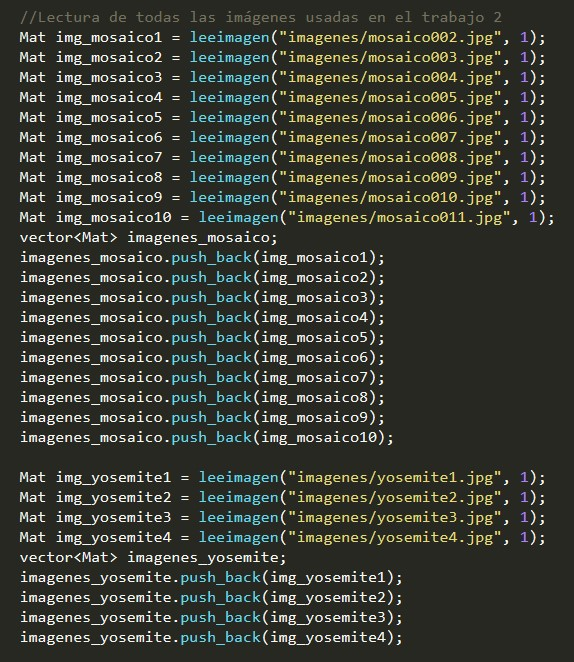
\includegraphics[width=0.7\linewidth]{lectura_im}
\caption{Lectura imagenes}
\end{figure}

Para continuar llamando a la función que ejecuta el ejercicio 1. Esta función realiza las siguientes acciones:

\begin{itemize}
	\item A la imagen pasada como parámetro, se le aplica la función de OpenCV cornerHarris para obtener en cada posición de la matriz resultado un valor Harris, cuanto mayor sea el valor obtenido más probabilidad hay de que ese valor sea una esquina.
	
	\item Una vez obtenidos la lista de puntos Harris procedemos a normalizarlos para obtener unos valores mas simplificados (función normalize de OpenCV)
	
	\item Ahora deberíamos, de esos valores obtenidos, eliminar aquellos que no son máximos locales con el fin de que no salgan puntos Harris en posiciones cercanas. Después de intentarlo durante mucho tiempo no he conseguido realizar la función no-maximo debido a no poder solucionar un fallo de segmentación. Por tanto, los resultados finales no serán del todo correctos y algunos puntos Harris se superpondrán.
	
	\item Ahora, la matriz que contiene los puntos Harris la transformamos en una lista ordenada de mayor a menor valor. Esto lo hacemos para, una vez ordenada, poder seleccionar solamente aquellos puntos con un buen valor Harris.
	
	\begin{figure}[H]
\centering
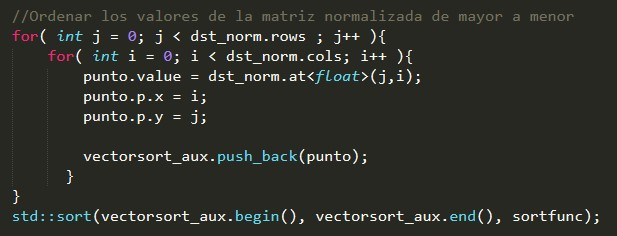
\includegraphics[width=0.7\linewidth]{matrizTovector}
\caption{Matriz harris a vector ordenado}
\end{figure}

	
	\item Por último nos quedaría seleccionar solamente los 1500*0.7 primeros valores de la lista creada en el punto anterior
	
\end{itemize}

Una vez realizado todo el proceso con la imagen original lo vamos a volver a repetir dos veces mas, cada una a partir de la imagen anterior escalada a la mitad (para ello usamos la función pyrDown de OpenCV) y seleccionando el 20\% y el 10\% de los puntos Harris obtenidos respectivamente.\\ 

Por último dibujamos un círculo en cada posición del vector que contiene todos los puntos Harris seleccionados.

\begin{figure}[H]
\centering
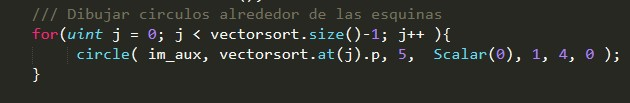
\includegraphics[width=0.7\linewidth]{dibujar_circulos}
\caption{Dibujado de circulo en cada punto Harris}
\label{fig:dibujarcirculos}
\end{figure}

La estructura principal del código de obtención de puntos Harris ha sido obtenida de un ejemplo de la documentación de OpenCV.\footnote{\url{http://docs.opencv.org/2.4/doc/tutorials/features2d/trackingmotion/harris_detector/harris_detector.html}}\\
\\
\subsection{Salidas obtenidas}

\begin{figure}[H]
\centering
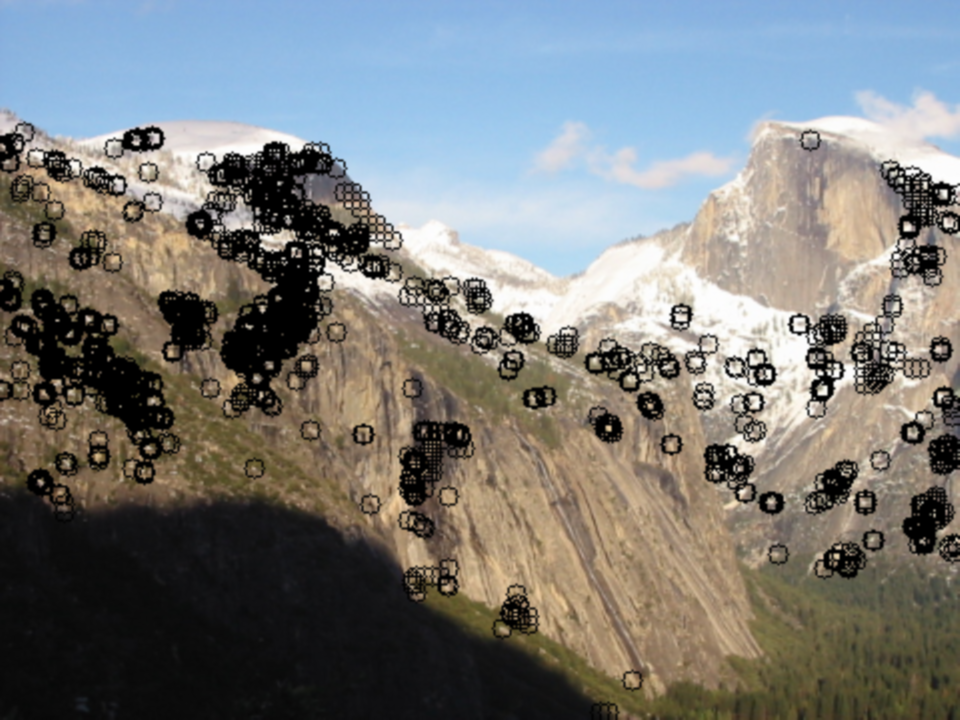
\includegraphics[width=0.7\linewidth]{Salida_ej1}
\caption{Puntos Harris obtenidos}
\label{fig:salidaej1}
\end{figure}

Como hemos comentado anteriormente, a los puntos Harris faltaría añadirle un método para eliminar los no-maximos locales, por lo que aunque en el resultado se muestran los puntos Harris de mayor valor este no es un resultado de calidad.

\newpage
\section{Ejercicio 2}

\subsection{Enunciado}

 Usar los detectores OpenCV (KAZE/AKAZE) sobre las imágenes de Yosemite.rar. Extraer extraer sus listas de keyPoints y establecer las correspondencias existentes entre ellas ( Ayuda: usar la clase DescriptorMatcher y BFMatcher de OpenCV). Valorar la calidad de los resultados obtenidos bajo el criterio de correspondencias OpenCV BruteForce+crossCheck. (1.5 puntos)

\subsection{Comentarios sobre el desarrollo}

Para realizar este ejercicio en primer lugar creamos una función con los siguientes parámetros de entrada:

\begin{figure}[H]
\centering
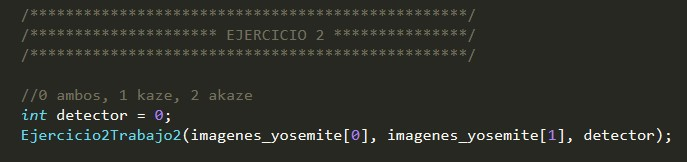
\includegraphics[width=0.8\linewidth]{cabecera_ej2}
\caption{Parámetros de entrada función ejercicio 2}
\label{fig:cabeceraej2}
\end{figure}

Como podemos ver la función recibe las dos imágenes a relacionar y un entero que determina si usamos el detector KAZE, el AKAZE o ambos.

En cuanto a la función de este ejercicio esta tiene dos partes: un calculo de los puntos en correspondencia mediante el detector KAZE y otro cálculo similar pero usando el detector AKAZE. Como la metodología a seguir en ambos ha sido la misma salvo el cambio de detector únicamente explicaré lo concerniente al detector KAZE.

Calculo de los puntos en correspondencia mediante el detector AKAZE
	
	\begin{figure}[H]
\centering
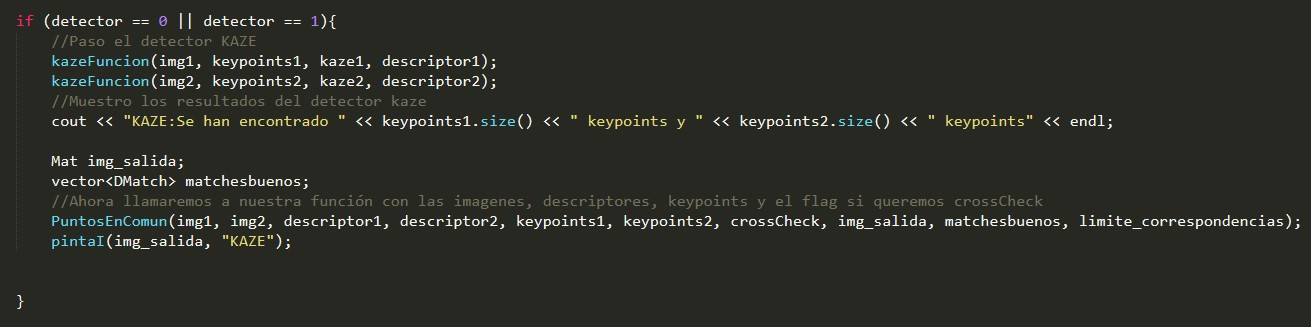
\includegraphics[width=0.8\linewidth]{codigokaze}
\caption{Código principal usando detector KAZE}
\label{fig:codigokaze}
\end{figure}

Esta función realiza lo siguiente: en primer lugar calculamos la lista de puntos clave y los descriptores de cada una de las dos imágenes para, una vez obtenidos estos valores pintar los puntos clave en la imagen original

\begin{figure}[H]
\centering
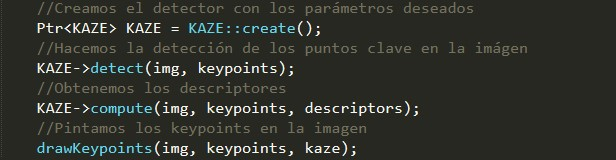
\includegraphics[width=0.8\linewidth]{codigokaze_sub}
\caption{Cálculo de los keypoints y descriptores}
\label{fig:codigokazesub}
\end{figure}

Ahora resta detectar y pintar los puntos en común entre ambas imágenes. Esto lo realiza la función PuntosEnComun que recibe las \textbf{dos
imágenes}, los \textbf{descriptores} y \textbf{keypoints} obtenidos anteriormente por los detectores, un booleano llamado \textbf{crossCheck} que indica si queremos que los valores obtenidos se realicen mediante el criterio de fuerza bruta o el de validación cruzada, la \textbf{imagen de salida} que devolverá las correspondencias entre ambas imágenes, \textbf{un vector} para devolver las correspondencias que hay entre ambas imágenes y un limite
\textbf{limite\_correspondencia} que explicaré mas adelante.

\begin{figure}[H]
\centering
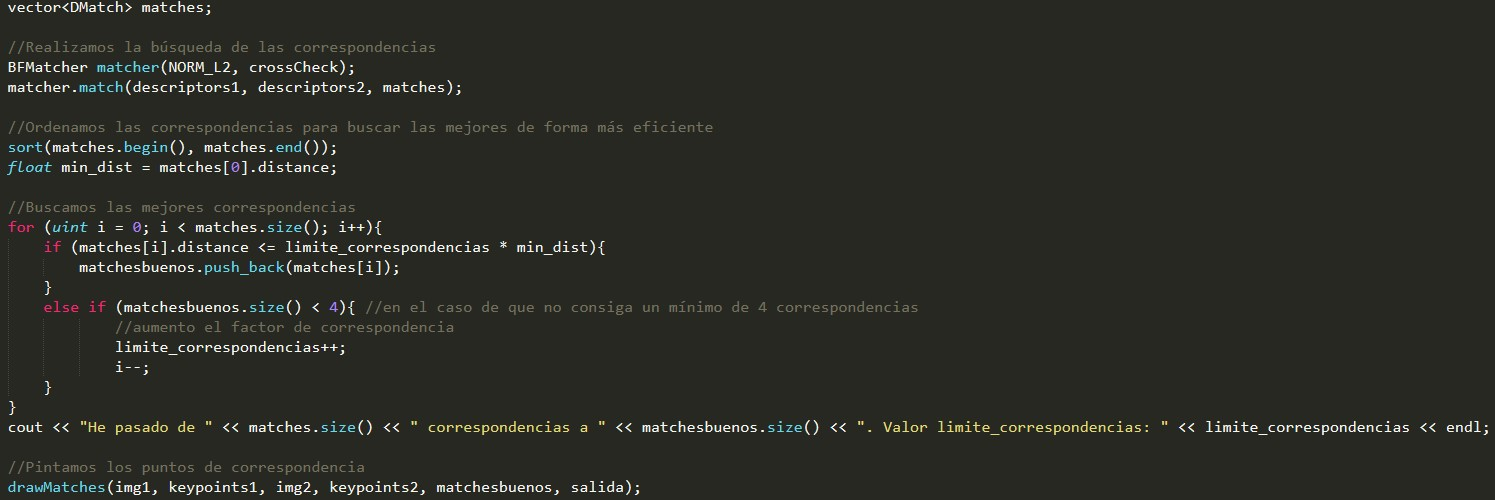
\includegraphics[width=1\linewidth]{puntosencomun}
\caption{Función para determinar los puntos en comun entre dos imagenes}
\label{fig:puntosencomun}
\end{figure}

En primer lugar realizamos la búsqueda de correspondencias y las ordenamos. Una vez tenemos todas las correspondencias vamos a determinar cuales de ellas son las mejores, para ello usamos el limite correspondencia. Lo que hace este limite es que solamente elijamos aquellas correspondencias cuya distancia sea cercana, las correspondencias  De esta forma las que tengan una distancia muy lejana las descartaremos por intuir que serán malas. Por ultimo un añado if de control para que si el numero de correspondencias buenas obtenidas es bajo relajar la restricción de la distancia aumentando el limite de correspondencia.\\

Ya sólo quedaría dibujar las correspondencias con la función drawMatches de OpenCV.

\subsection{Salidas obtenidas}

\begin{figure}[H]
\centering
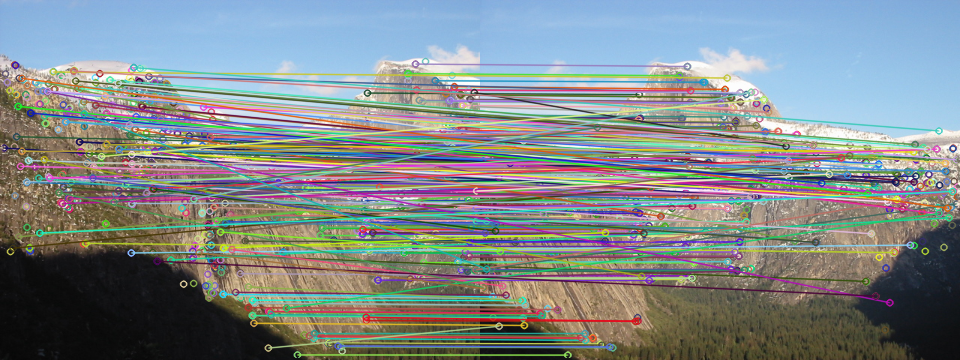
\includegraphics[width=1\linewidth]{ej2_kaze}
\caption{Correspondencias usando KAZE, crossCheck activado y limite de correspondencia 1}
\label{fig:ej2kaze}
\end{figure}

\begin{figure}[H]
	\centering
	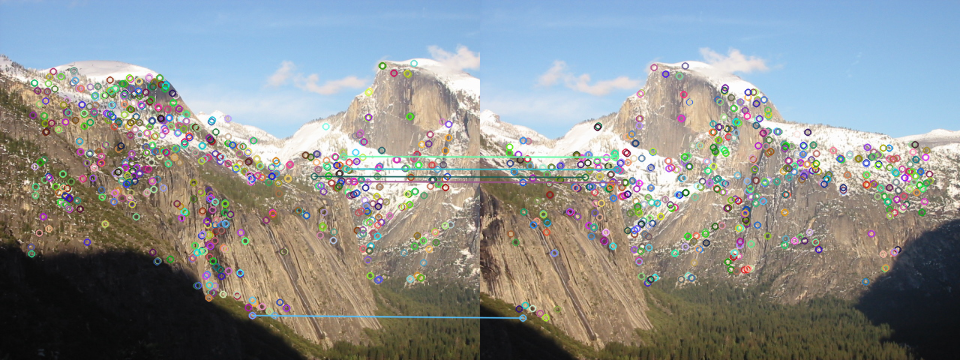
\includegraphics[width=1\linewidth]{ej2_akaze}
	\caption{Correspondencias usando AKAZE, crossCheck activado y limite de correspondencia 1}
	\label{fig:ej2akaze}
\end{figure}

\begin{figure}[H]
\centering
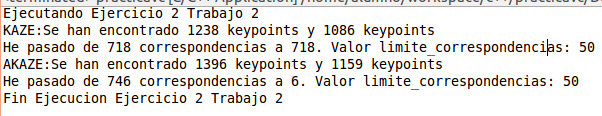
\includegraphics[width=0.7\linewidth]{salidaTextoEj2}
\caption{Datos obtenidos ejercicio 2}
\label{fig:salidatextoej2}
\end{figure}


Como podemos ver, el limite de correspondencia influye a la hora de determinar las correspondencias en el caso de AKAZE, mostrándonos sólo las 5 más prometedoras.

\newpage
\section{Ejercicio 3}

\subsection{Enunciado}

(OPCION: 10 puntos) Escribir una función que forme un Mosaico de calidad a partir de N > 3 imágenes relacionadas por homografías, sus listas de keyPoints calculados de acuerdo al punto anterior y las correspondencias encontradas entre dichas listas. Estimar las homografías entre ellas usando la función findHomography(p1,p2,CV\_RANSAC,1). Para el mosaico será necesario.\\
\\
a) definir una imagen en la que pintaremos el mosaico; b) definir la homografía que lleva cada una de las imágenes a la imagen del mosaico; c) usar la función warpPerspective() para trasladar cada imagen al mosaico (ayuda: mirar el flag BORDER\_TRANSPARENT de warpPerspective para comenzar). (4 puntos)

\subsection{Comentarios sobre el desarrollo}

La función de este ejercicio recibirá como argumentos un vector con todas las imágenes que forman el mosaico, las dimensiones máximas del mosaico y el limite de correspondencia explicado en el punto anterior.\\

Lo primero que hacemos es mostrar por pantalla todas las imágenes que van a formar parte del mosaico para, a continuación, llamar a la función crearSuperMosaico, que será la encargada de ir añadiendo cada una de las imágenes al mosaico de la siguiente forma:

\begin{figure}[H]
	\centering
	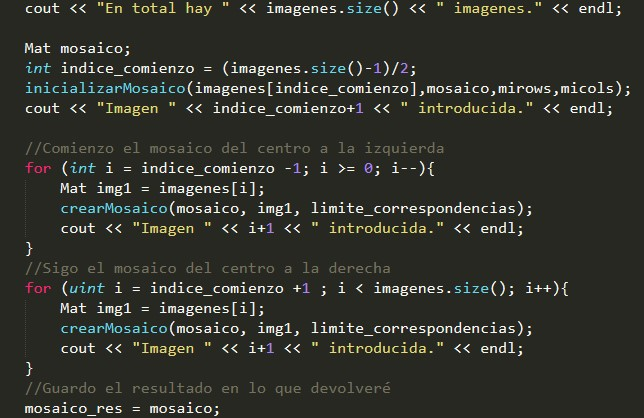
\includegraphics[width=0.7\linewidth]{supermosaico}
	\caption{Código de la función principal que crea el mosaico}
\end{figure}

Esta función en primer lugar inicializa el mosaico con las dimensiones introducidas y colocando la primera imagen (que será la que esté en el centro del vector de imágenes).\\

A continuación voy recorriendo el vector de imágenes primero hacia la izquierda y luego hacia la derecha y llamando a la función encargada de determinar los keypoints, las correspondecias entre el estado actual del mosaico y la nueva imagen a introducir para acabar buscando la homografia de la lista de keypoints de ambas imágenes. Por ultimo, con la función wrapPerspective realizamos las transformaciones de la imagen que la homografía calculada previamente nos indica.

\begin{figure}[H]
	\centering
	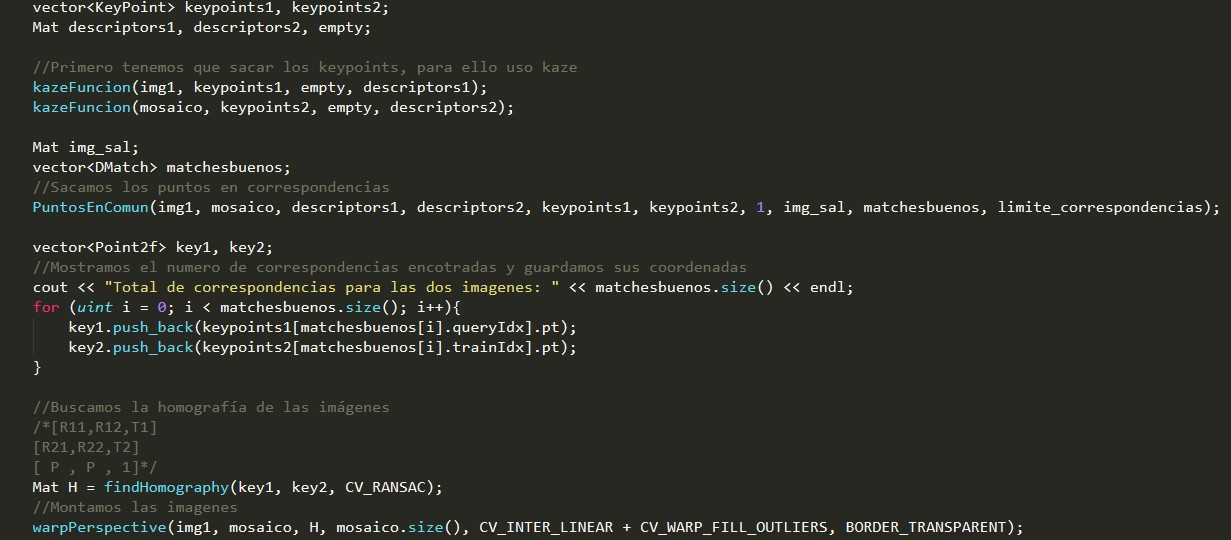
\includegraphics[width=0.7\linewidth]{mosaico}
	\caption{Código de la función que calcula todo lo necesario para unir una imagen de entrada con el mosaico principal}
\end{figure}


\subsection{Salidas obtenidas}

\begin{figure}[h]
\centering
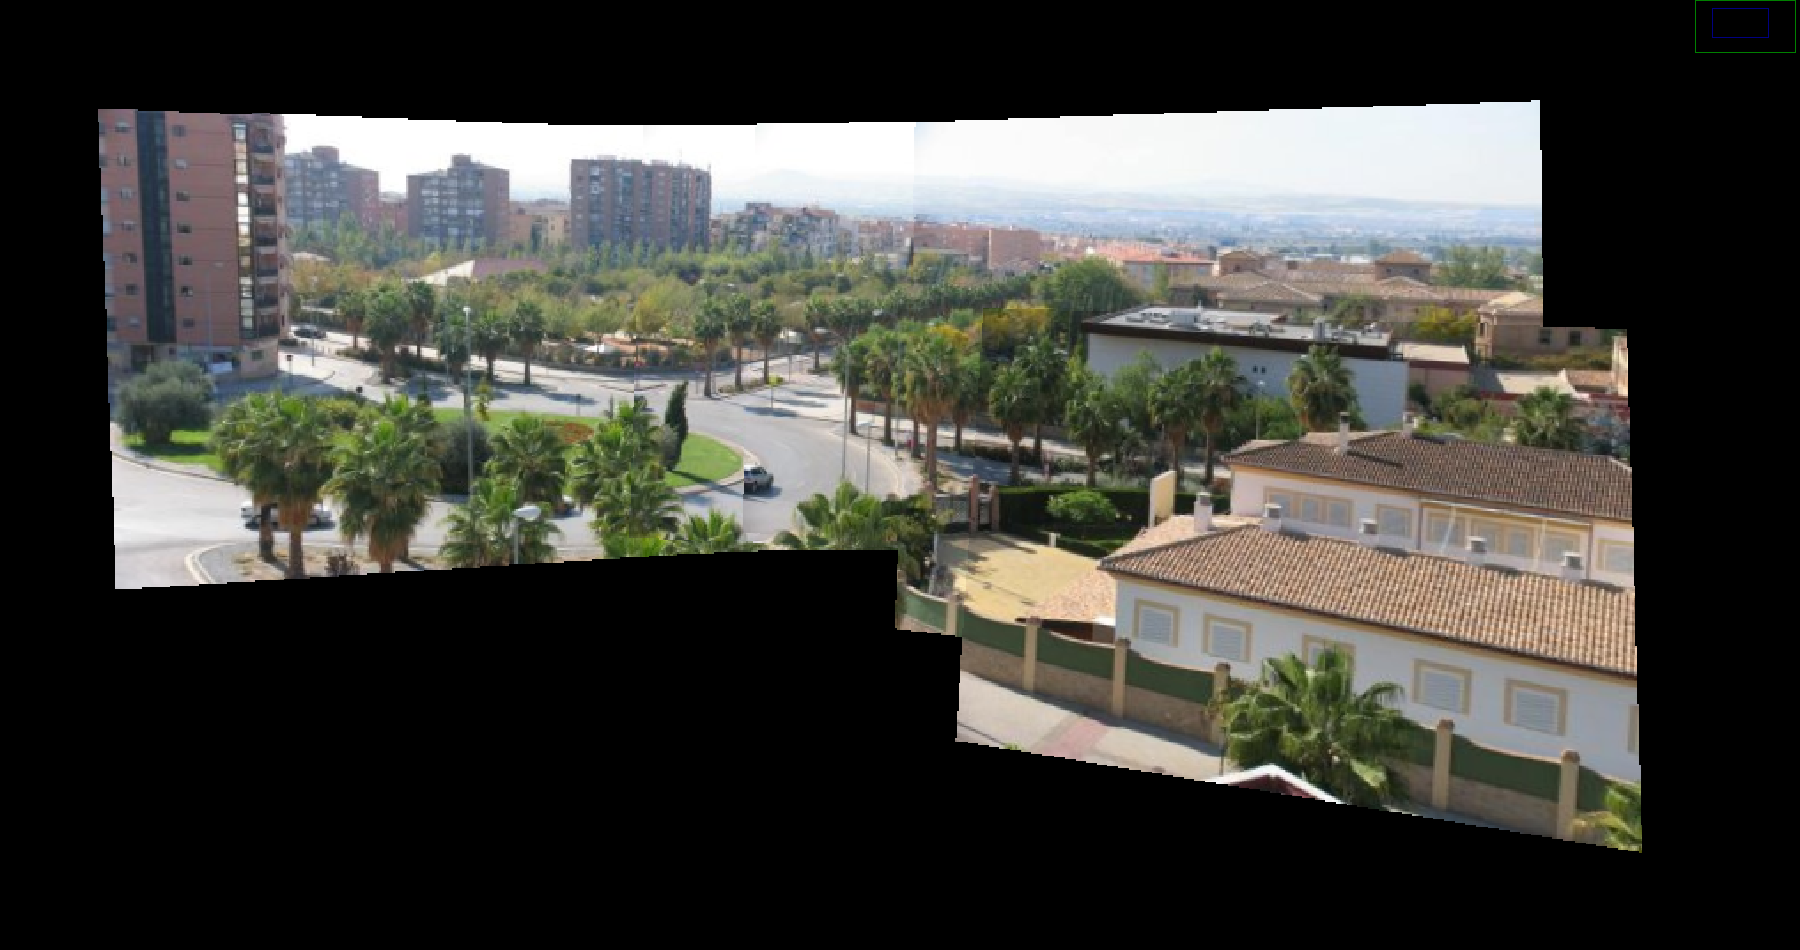
\includegraphics[width=1\linewidth]{salidaEj3Etsiit}
\caption{Mosaico ETSIIT}
\label{fig:salidaej3etsiit}
\end{figure}

\begin{figure}
	\centering
	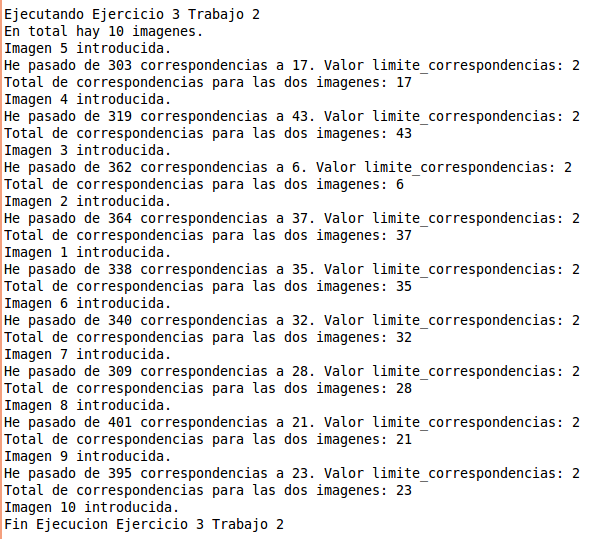
\includegraphics[width=0.7\linewidth]{salidaTextoEj3_etsiit}
	\caption{Salida texto mosaico ETSIIT}
	\label{fig:salidatextoej3etsiit}
\end{figure}


\begin{figure}[H]
\centering
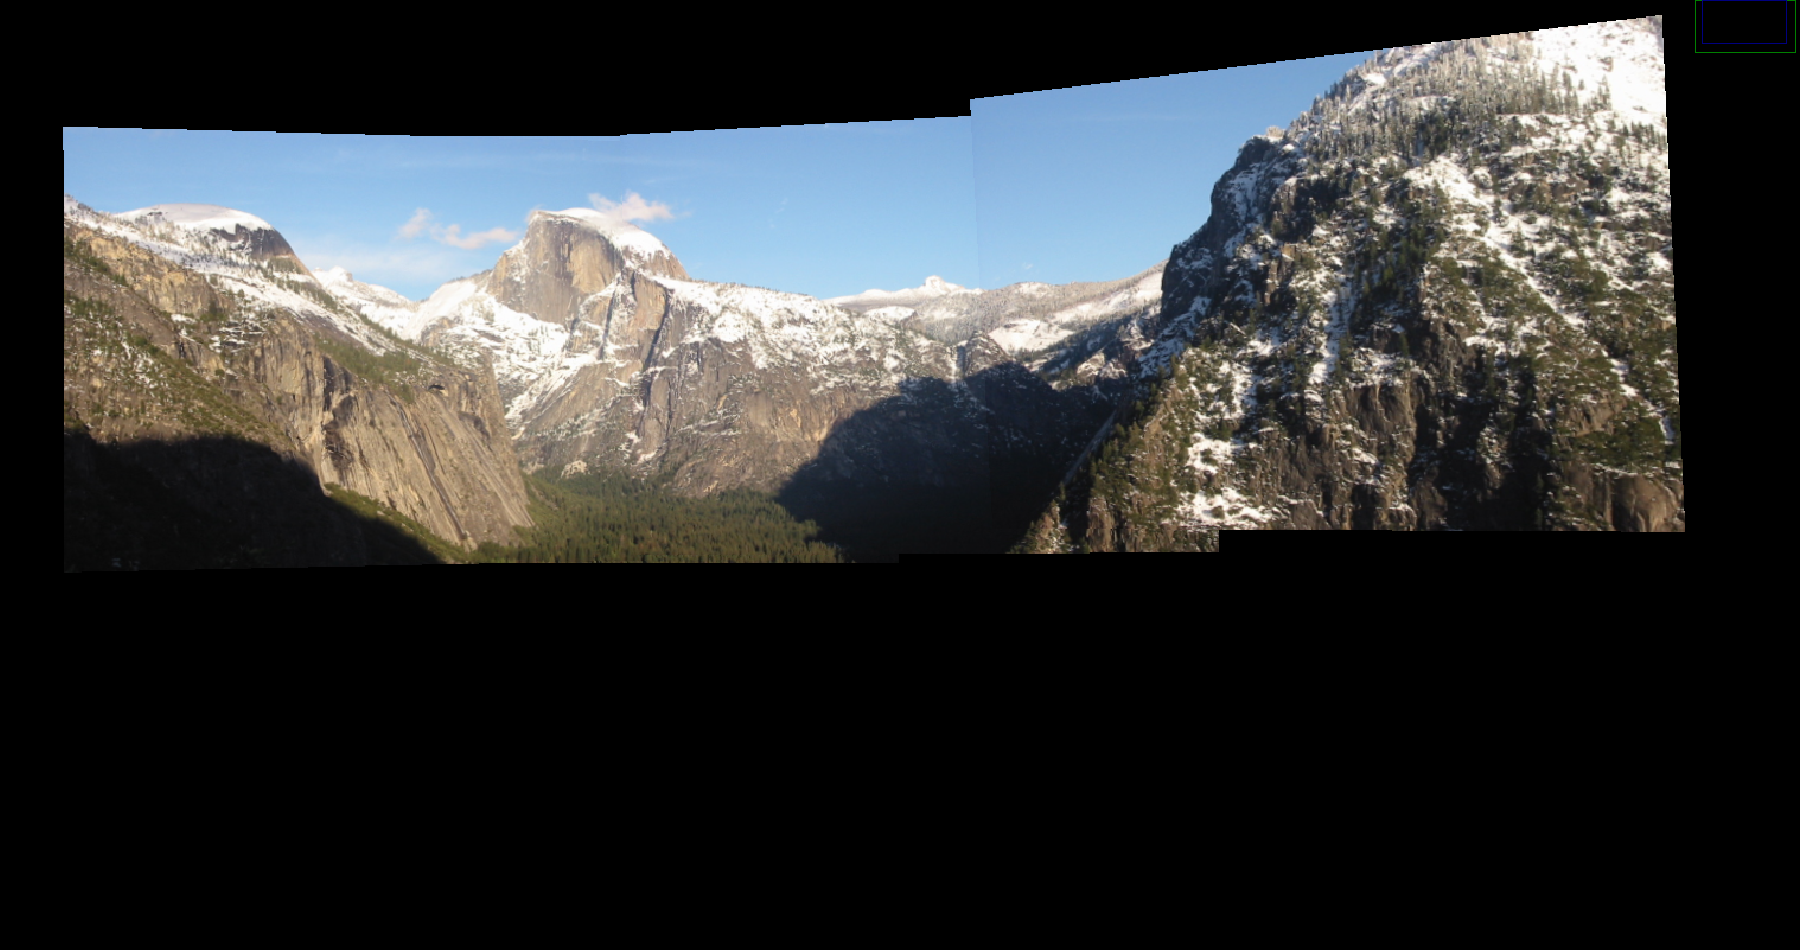
\includegraphics[width=1\linewidth]{salidaEj3Yosemite}
\caption{Mosaico Yosemite}
\label{fig:salidaej3yosemite}
\end{figure}

\begin{figure}[H]
\centering
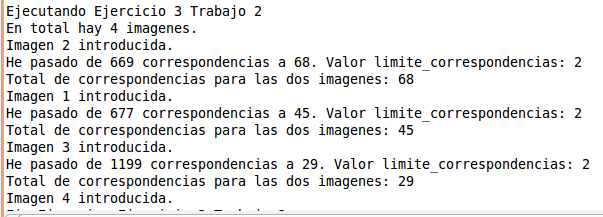
\includegraphics[width=0.7\linewidth]{salidaTextoEj3_yosemite}
\caption{Salida texto mosaico yosemite}
\label{fig:salidatextoej3yosemite}
\end{figure}

Como podemos ver ambos resultados son razonablemente buenos.

\end{document}